\section{Introduction}
\label{sec:intro}

\IEEEPARstart{D}{rone} inspection of wind-turbine blades is one of the most mature industrial applications of visual defect detection. Blades erode at the leading edge, crack, delaminate, collect dirt and oil, and are struck by lightning, and an operator needs to find these defects early, before they grow into structural damage. Unmanned aerial vehicles (UAVs) capture thousands of close-range photographs per turbine, and deep detectors are expected to sort them. The published numbers suggest that the problem is nearly solved. BladeYOLO~\cite{bladeyolo} reports 86.5/57.4 \mfifty/\mcoco on Wind Surface Defect and 85.8/74.6 on WTBlade-Defect. Other recent architectures, built on YOLO detectors with attention, wavelet, deformable or state-space modules, report similar levels~\cite{gfdyolox,gayolo,kgpyolo}.

This work began as an attempt to reproduce BladeYOLO and build on it. Our closest faithful reimplementation stopped at about 52.6/28.0. A heavier model of our own then reached 78.2/46.9, which looked like a breakthrough until we found that three-quarters of the validation images had a near-identical twin in the training set. That finding changed the question from ``how do we beat this number?'' to three others:
\begin{enumerate}
\item What do the public blade-defect benchmarks measure?
\item How much of a reported score is memorisation of scenes seen in training?
\item Once leakage is removed, what actually helps, and what limits the score?
\end{enumerate}

We answer them with an end-to-end audit and about two and a half months of controlled experiments, recorded in a public research log~\cite{repo}. From late October onwards every hypothesis was written down with its pass bar before any run, and committed~\cite{prereg}. After a bad result we allowed one scope check and then discarded the hypothesis, without rescue runs. The paper therefore reports the failures as well as the successes. Fig.~\ref{fig:pipeline} shows how the parts of the study fit together.

\begin{figure}[!t]
\centering
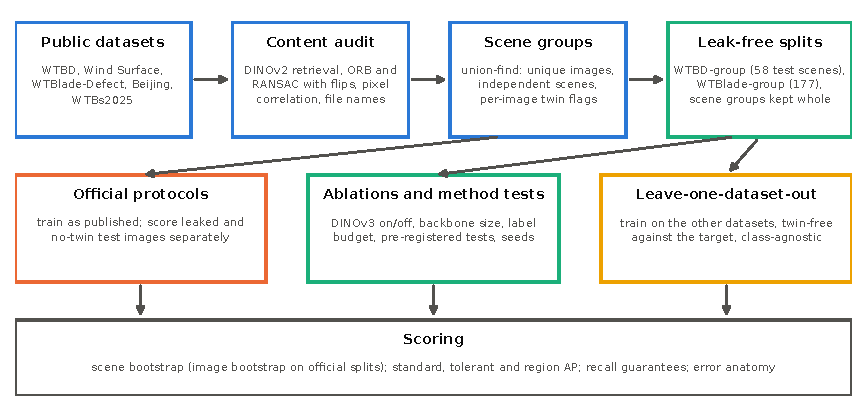
\includegraphics[width=\linewidth]{fig7_pipeline}
\caption{Overview of the study. The content-based audit produces scene groups and per-image twin flags. These define the leak-free splits (WTBD-group, WTBlade-group) and the leaked and no-twin subsets of the official test sets. Every experiment shares the same evaluator and scene bootstrap.}
\label{fig:pipeline}
\end{figure}

\subsection{Contributions}
\begin{itemize}
\item \textbf{A leakage audit of the public blade benchmarks} (Table~\ref{tab:audit}, Fig.~\ref{fig:twins}). We find twins for 78\%, 84\% and 92\% of the official test images of WTBD, Wind Surface and WTBlade-Defect. A literature check found no earlier audit of these datasets.
\item \textbf{A reproduction record of BladeYOLO} (Section~\ref{sec:history}, Fig.~\ref{fig:official-bladeyolo}). It explains why our reproduction gave different results: an unpublished split, a public copy with 220 fewer images, our own early code defects, and leakage.
\item \textbf{The size of the inflation}, measured with one detector and recipe. We compare leaked against no-twin test images (Table~\ref{tab:subsets}) and official against scene-grouped splits (Table~\ref{tab:split-only}). We also show that tuning on the official splits selects for memorisation (Table~\ref{tab:tuning}).
\item \textbf{Two leak-free benchmarks}, WTBD-group and WTBlade-group, with audited splits, scene groups, a scene bootstrap and baselines for four detector families (Table~\ref{tab:leakfree}).
\item \textbf{Controlled ablations} that attribute the advantage of a DINOv3-fused YOLO to the frozen features alone, across the learning curve and three backbone sizes (Tables~\ref{tab:ablation}, \ref{tab:backbone}).
\item \textbf{RF-DETR-FP}, a detection transformer with a frozen DINOv3 prior beside its fine-tuned encoder, motivated by measured feature drift and encoder collapse. It was tested under a pre-registered paired protocol on leak-free and official splits (Section~\ref{sec:fp-results}).
\item \textbf{Measured ceilings}: annotator self-consistency, box granularity, subset luck and error anatomy (Section~\ref{sec:why}).
\item \textbf{A leave-one-dataset-out test} with twin-free pools (Section~\ref{sec:lodo}), and \textbf{a recall-guarantee failure} caused by leaked calibration (Table~\ref{tab:conformal}).
\item \textbf{A ledger of the method tests} we ran or formally gated, including the failures (Table~\ref{tab:ledger}).
\end{itemize}

The authors of the papers we discuss followed common practice, which is to augment and then split at random. Our argument is about the protocol, not about them. We cannot say that any specific published number is due to memorisation, because those splits were not published.

\subsection{Organisation}
Section~\ref{sec:related} reviews related work. Section~\ref{sec:audit} presents the datasets and the leakage audit, and Section~\ref{sec:benchmarks} the leak-free benchmarks and the evaluation protocol. Section~\ref{sec:models} describes the detectors, including the proposed RF-DETR-FP. Section~\ref{sec:official} reports the official protocols: the reproduction of BladeYOLO, our scores against the published ones and what those scores are made of. Section~\ref{sec:leakfree} gives the leak-free results and ablations, and Section~\ref{sec:why} explains why leak-free scores are low. Section~\ref{sec:lodo} tests whether external data replaces target labels, and Section~\ref{sec:failed} records what did not work. Section~\ref{sec:discussion} closes with recommendations, limitations and conclusions. The appendices give the project timeline (Appendix~\ref{app:timeline}), the conclusions we corrected along the way (Appendix~\ref{app:corrections}), the engineering defects that affected results (Appendix~\ref{app:engineering}) and the per-class audit and full run registry (Appendix~\ref{app:registry}).
